\subsection{Schwarzschild modes \textbf{N}}
	We now have a look at free fields in the Schwarzschild geometry. For the beginning we need to find a set of modes $f$ that solve the free scalar equation of motion:
		\begin{equation} \label{Klein_Gordon_curved}
			\frac{1}{\sqrt{-g}} \partial_\mu (\sqrt{-g} g^{\mu \nu} \partial_\nu \phi)
			= m^2 \phi
		\end{equation}
	which is the \textit{Klein-Gordons equation for curved space} and where $g_{\mu \nu}$ is the Schwarzschild metric and $g$ is its determinant. Its solutions are also modes in \eqref{wave_fct}, were we can study its properties in an appropriate quantum state such as the Hartle-Hawking state\footnote{The Hartle-Hawking state is the pure state for the Schwarzschild geometry, where the two exteriors of the Rindler space are thermally entangled as seen in the chapter \ref{approxChap} above.}
	
	We now focus on the right exterior of the Schwarzschild geometry, where we use the coordinates $(t,r, \Omega)$. The solutions are having the form
		\begin{equation}
			f_{\omega l m} = 
			\frac{1}{r} Y_{l m}(\Omega) e^{-i \omega t} \psi_{\omega l}(r)
		\end{equation}
	Let's put these into the equation \eqref{Klein_Gordon_curved} above, use the tortoise coordinates from \eqref{r_*tortoise} and plug in
		\begin{align*}
			g^{\mu \nu} &= diag \left(
				\frac{1}{\frac{1}{r}-1},
				1 - \frac{1}{r},
				\frac{1}{r^2},
				\frac{1}{r^2 \sin \theta}
			\right) \\
			\Rightarrow \sqrt{-g}&= r^2 \sin \theta
		\end{align*}
	to reform it into a Schrödinger equation:
		\begin{equation}
			- \frac{d^2}{dr^2_*} \Psi_{\omega l} 
			+ V(r) \Psi_{\omega l} 
			= \omega^2 \Psi_{\omega l}
		\end{equation}
	with the effective Potential of
		\begin{equation}
			V(r)=
			\frac{r-1}{r^3} \left( m^2r^2 + l(l+1) + \frac{1}{r}
			\right)
		\end{equation}
	Let's have a look at the mass m: For simlicity, we consider the Compton wavelength $\frac{1}{m}$ can be\footnote{ The \textit{Schwarzschild radius $r_s$ is still 1}, but I sometimes write $r_s$ to make some things better understandable.} 
		\begin{enumerate}[(i)]
			\item $\frac{1}{m} \ll r_s$	~~ which is the \textit{massive case} and \label{massive}
			\item $\frac{1}{m} \gg r_s$	~~ which is the \textit{massless case}. \label{massless}
		\end{enumerate}
	For to explain, why case \eqref{massless} is more interesting for us, we first need to have a look at case \eqref{massive}.
	
	Here the potential goes to $m^2$ for $r \gg 1$ which means that massive modes will only propagate till near infinity if $\omega \geq m$. Because we assumed, that $m \gg 1$, any modes with an energy $\omega$ of order of the Schwarzschild radius \textit{will stay near the horizon}. 
	 
	But we found out earlier, that the temperature of black holes is of order $\frac{1}{r_s}$. This means, that $\omega \approx 1$ would be the most interesting energy, but if the mass is already much bigger than one, we cannot examine the propagation to infinity because $\omega$ would also be much bigger than one.
	
	\begin{figure} [tbp]
			\begin{center}
				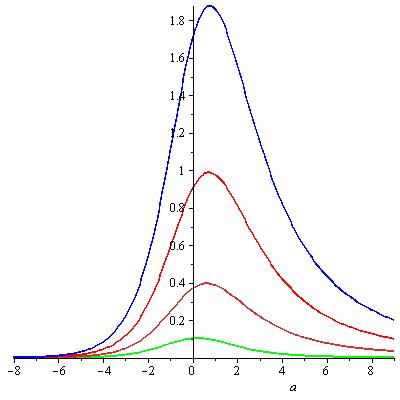
\includegraphics[scale=0.5]{plots_of_V}
				\caption{These are the selvemade plots of $V(r_*)$ for $l=\{0,1,2,3$\}.} \label{plots_of_V}
			\end{center}
	\end{figure} %eigener Plot eingefügen
		
	So from now on we remain within the case of $m^2=0$, the massless case.
	Here the asymptotic behavior of the potential is
		\begin{equation} \label{potential_near_infinity}
			V\approx
			\begin{cases}
				\frac{l(l+1)}{r^2_*} &r_* \rightarrow \infty \\
				(l^2 + l + 1) e^{r_*-1} &r_* \rightarrow - \infty
			\end{cases}
		\end{equation}
	If you wonder, why $r_*$ can go to infinity, then send $r$ in the tortoise coordinate \eqref{r_*tortoise} to 1 (which would be the Schwarzschild radius). You will get minus infinity. So this just means, that $r$ approaches $r_s$. 
	
	So the first approachment in \eqref{potential_near_infinity} leads to the vanishment of the potential at spatial infinity polynomially in $r_*$, but near the horizon it vanishes exponentially.
	The barrier between these two regions of \eqref{potential_near_infinity} can be seen in \textbf{Figure \ref{plots_of_V}}. For $\ell \gg 1$ we will find the peak at $r_* = \frac{3}{2}$ with a height of order $\ell$.
	
	 	
	\begin{figure} [tbp]
		\begin{center}
			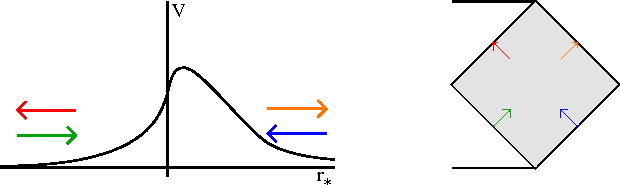
\includegraphics[scale=1.6]{schscat}
			\caption{Bla} 
		\end{center}
	\end{figure}